\section{평가 체계}
\label{sec:eval}

\begin{figure*}[t]
\centering
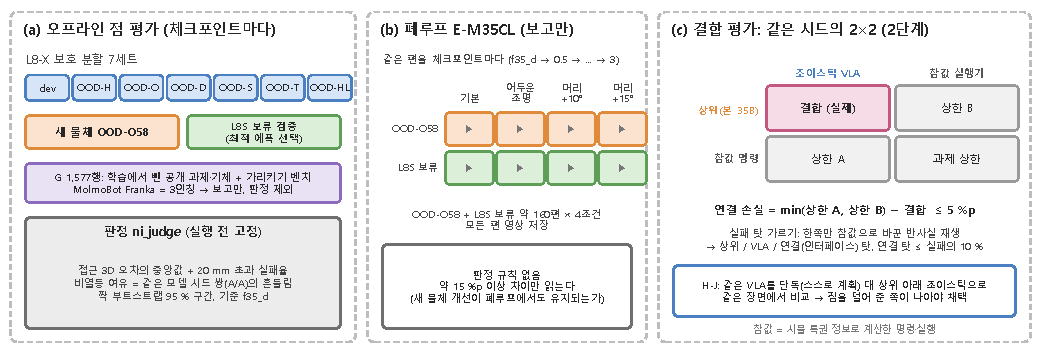
\includegraphics[width=\linewidth]{figures/eval_protocol.pdf}
\caption{\textbf{평가 체계.} (a) 체크포인트마다 오프라인 점 평가. (b) 폐루프 E-M35CL(보고 전용). (c) 결합 평가: 같은 시드 2$\times$2와 원인 분리, H-J 비교. 참값은 시뮬 특권 정보로 계산한 명령·실행이다.}
\label{fig:eval}
\end{figure*}

\paragraph{오프라인 점.} L8-X 보호 분할 7세트(dev\_x, 본 적 없는 탁자 높이 OOD-H, 리프트 범위의 보류 높이 OOD-H-lift, 새 물체 범주 OOD-O, 보류 방해물·재질·조명 OOD-D, 보류 조합 OOD-T, 보류 가구 OOD-S), 학습에 한 번도 나오지 않은 실물 13종의 새 물체 세트 OOD-O58(\tentative{58}편), L8S 보류 검증, 일반 평가 G(학습에서 뺀 공개 과제·기체와 공개 가리키기 벤치, 1,577행)를 쓴다(\cref{fig:eval}a). G의 MolmoBot Franka 세트는 전부 3인칭·어안이라 보고만 하고 판정에서 뺀다. 지표는 접근 목표 3D 오차의 중앙값과 20\,mm 초과 실패율이다. 비열등 여유는 같은 모델의 두 시드(A/A) 흔들림으로 정하고, 같은 스냅숏 짝 부트스트랩 95\,\% 구간으로 판정한다.

\paragraph{폐루프.} 새 물체 OOD-O58과 L8S 보류 편을 기본, 어두운 조명, 머리 기울기 +10$^\circ$·팬 +15$^\circ$ 변형으로 체크포인트마다 돌린다(E-M35CL, \cref{fig:eval}b). 편당 한 번이라 약 15\,\%p 이상의 차이만 읽는 보고 전용이며, 모든 편의 머리·손목 영상을 저장한다.

\paragraph{결합.} 같은 시드 2$\times$2로 연결 손실과 원인 비율을 재고(\cref{sec:closs}), 같은 VLA를 단독 모드와 조이스틱 모드로 돌려 H-J를 비교하며, 판당 대기 시간·취소율을 함께 적는다(\cref{fig:eval}c). 세트는 새 물체, L8S 보류, L9 보류다.

\paragraph{절차.} 모든 실험은 ``이 결과로 바꾸는 결정''과 판정 규칙을 실행 전에 사전 등록한다. 판정 규칙을 바꾸면 등록 문서에 변경으로 남기고, 관문을 넘기는 결정은 기록과 함께 사람이 한다.
